\chapter{Introduction}
\label{chap:introduction}

\section{Context}
\label{sec:context}

There is no doubt about the importance of online video streaming.
According to Sandvine \cite{sandvine1},
in 2020, 57\% of the global internet traffic was used by video streaming.
Moreover, one of the key predictions made by Cisco in 2018 \cite{cisco1}
stated that by year 2022, video traffic will make up 82\% 
of all \textit{IP} traffic.


Consequently, many challenges arise. Due to the growth in the 
number and diversity of connected video-capable devices, and the 
increasing bandwidth and higher quality content available, the
video client needs to adapt the multimedia content to
the network and the devices. The technique of taking account the 
varying network conditions and computing resources of the user 
device to choose the adequate quality level is denominated as
\textit{Adaptive BitRate (ABR)}. Adaptation may be performed by
monitoring different parameters such as estimated bandwidth,
client's buffer level, CPU load or screen size.


The \textit{Dynamic Adaptive Streaming over HTTP (DASH)} is the
standard that implements adaptive bitrate video streaming and was developed
by the \textit{Moving Picture Experts Group (MPEG)} \cite{dash1}. \textit{MPEG-DASH} 
enables provisioning and delivering media using existing \textit{HTTP}-delivery 
networks supports dynamic adaptation with seamless switching. By using
\textit{HTTP}, the player will not have firewall problems. The quality selection 
relays on the client thus providing better scalability.

  
\begin{figure}[h]
  \label{fig:chart1}
    \centering
    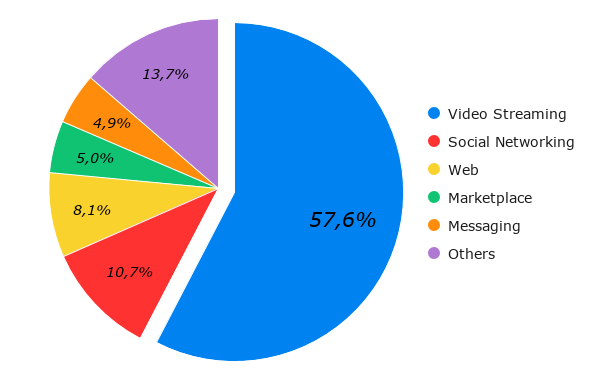
\includegraphics[width=0.85\textwidth]{img/chart2.png}
    \caption{Global application category total traffic share during COVID-19 lockdown. Source: Sandvine \cite{sandvine1}}
  \end{figure}
  
  
The \textit{MPEG-DASH} standard was published in 2012 and revised in 2019 
by the \textit{International Organization for Standardization (ISO) / International 
Electrotechnical Commission (IEC)} as \textit{MPEG-DASH ISO/IEC 23009-1:2019}
\cite{ISO23009}. In addition, the \textit{3\textsuperscript{rd} Generation Partnership Project (3GPP)}
defines the use of \textit{DASH} as the standard continuous for delivering of multimedia
content in mobile networks, specifically in \textit{LTE} and 5G networks \cite{3gpp1}.

\textit{DASH} splits the input stream into small chunks or segments
which are defined in the the \textit{Media Presentation Description (MPD)}, 
which is an XML manifest file that contains the \textit{Universal Resource 
Locators (URL)} of the segments. The \textit{MPD} contains information for each 
representation such as the codec, bandwidth, resolution or framerate.
Different qualities are defined as representations.

However, the DASH Standard \cite{ISO23009} only defines the data formats
for the media reproduction and do not provide any description on the adaptation algorithm.
This thesis will analyze and compare a small number of adaptation algorithms.
The \textit{DASH Industry Forum} \cite{dash2} provides an open source \textit{MPEG-DASH} 
player implemented in \textit{JavaScript} with different adaptation algorithms.
Similarly, \textit{hls.js} is an implementation of a \textit{HTTP Live Streaming}\footnote{HTTP
Live Streaming is a HTTP-based adaptive bitrate streaming protocol developed by Apple Inc.
 \cite{hls1}} client.

The adaptation algorithms needs to be tested in different scenarios (they can be simulated)
and be tweaked to provide the maximum perceived quality by the users. Also, there are
algorithms that perform better in some specific scenarios and worse in others. The adaptation
algorithm is the responsible for avoiding problems that may have a negative impact
on the \textit{Quality of Experience (QoE)} such as service disrruption or
frequent changes on the bitrate. 
One problem is that, the algorithm can overestimate
the bandwidth, this means requesting segments of a superior quality that the channel can support,
and it would cause a pause in the reproduction because all the 
segments in the buffer are emptied. The algorithm can also underestimate the bandwidth,
the video player requests media segments with inferior quality than the quality at which the 
bandwidth available of the network can allow. Lastly, the algorithm should avoid
constant bitrate switches result of bandwidth fluctuations, and provide a smooth and
seamless video watching experience.

This project will study and analyze the adaptation algorithms using \textit{}
The \textit{ns-3} simulator is an open-source and extensible discrete-event network simulator. 
The extensible nature of this tool allows us to develop a new module for \textit{ns-3}
mimicking the behaviour of \textit{ABR} clients and servers. With this new module, \textit{ns-3} 
will be able to simulate diverse mobile network scenarios and test the performance of adaptation algorithms.



\section{Objectives}
\label{sec:objectives}
The objectives of this thesis is to build a framework for testing \textit{ABR} adaptation
algorithms, and implement some adaptation algorithms and compare them in 
various mobile network scenarios with different objective \textit{QoE} metrics. 
In order to achieve the proposed objectives, the following steps will be proposed:

\begin{enumerate}
  \item Study and understand \textit{ns-3} and basic modules such as the core module, the
  internet module, applications module, \textit{LTE} module among others. Build basic \textit{LTE} scenarios
  tweak radio parameters, and output results.
  \item Design a new module in \text{ns-3} that simulates behaviours of \textit{ABR} clients
  and servers. Study and implement existing adaptation algorithms.
  \item Obtain objective \textit{QoE} and \textit{QoS} metrics.
  Build new \textit{LTE} scenarios and compare the performances of the implemented adaptation
  algorithms.
\end{enumerate}


\section{Structure of the thesis}
\label{sec:structure}

% The memory of this work is structured as follow:

\textbf{\textit{Chapter 1.}} Presents the context, the motivations and the objectives of this thesis.

\textbf{\textit{Chapter 2.}} The State of the Art. Includes an introduction to ABR and DASH. The architecture
and video quality adaptation algorithms. Also, an brief explaination of LTE, its architecture and fundamentals.

\textbf{\textit{Chapter 3.}} A starting guide to use \textit{ns-3}. Brief introduction and usage of 
relevant \textit{ns-3} modules for this thesis.

\textbf{\textit{Chapter 4.}} Introduces a new module for \textit{ns-3}, the \textit{ABR} module. Describes components 
and models of the \textit{ABR} module. Highlights the implemented adaptation algorithms.

\textbf{\textit{Chapter 5.}} Goes through a set of testing scenarios. Analyses and compares the different implemented adaptation algorithms.

\textbf{\textit{Chapter 6.}} Concludes the thesis and discusses possible future works.
